\part{Plateforme du comportement des occupants}

\chapter{Simulation Stochastique à base d'agents (MASS)}
\label{MASS}

L'état de l'art sur la modélisation du comportement des occupants nous a amené à nous orienter vers une modélisation stochastique à base d'agents. Pour les raisons évoquées en chapitre \ref{Approches de modélisation} le travail réalisé dans la suite s'inscrit en collaboration et dans la continuité des travaux de MASS effectués par le département \textit{Building and Urban Physics and Head of the Energy and Sustainability Research Division} de l'Université de Nottingham. 

Ce chapitre présente dans un premier temps les concepts généraux de la co-simulation et de sa mise en place informatique, puis présente dans un second temps le fonctionnement de MASS dans l'environnement d'EnergyPlus.

\section{Concepts génériques}

% Points faibles BCVTB et middleware
Nous avons vu que la co-simulation entre plusieurs outils permet d'étendre leurs propres fonctionnalité. Coupler EnergyPlus, ou d'autre logiciels de simulation, avec des programmes externes a été réalisé dans le passé, soit en créant des interfaces spécifiques aux programmes externes dans le code source d'EnergyPlus \cite{Huang-99} soit en utilisant un middleware\footnote{un middleware est un logiciel tiers qui créer un réseau d'échange d'informations entre différentes applications informatiques} tel que le \textit{Buildings Controls Virtual Test Bed} (BCVTB) \cite{Wetter-11} \cite{Langevin-14} pour EnergyPlus. Les limitations principales de ces approches sont d'une part le manque de ré-utilisabilité, car l'interface est spécifique à un unique programme et d'autre part la complexité et le ralentissement du temps de calcul qu'implique l'usage d'un middleware.

% Histoire FMI
En 2013, Nouidui et al \cite{Nouidui-13} proposent de court-circuiter ce middleware en couplant directement EnergyPlus avec un programme externe, par l'utilisation de l'interface \textit{Functional Mockup Interface} (FMI). Ce travail démontre alors le potentiel de cette approche issue des travaux du projet européen MODELISAR - ITEA2 terminé en 2011 et chapeauté par Daimler AG et Dassault Systèmes. Dans le cadre de ce projet, Plessis et al. \cite{Plessis-14} ont par ailleurs couplé leur simulateur du comportement des occupants SMACH avec le logiciel Modelica. L'Annex 60: "\textit{New generation computational tools for building and community energy systems based on the Modelica and Functional Mockup Interface standards}" de l'Agence Internationale de l'Energie, se terminant en 2017, a été lancé avec comme objectif de renforcer l'intégration, la robustesse et la performance de ce standard FMI.

% C, C++
Hong al. \cite{Hong-16} et Chapman et al. \cite{Chapman-14} ont tout les deux choisi d'utiliser le standard FMI pour co-simuler EnergyPlus avec une plateforme de modélisation de comportement des occupants. Alors que Hong et al. ont choisi de développer en C, Chapman et al. ont développé leur plateforme de comportements en C++. Cette différence minime de langage, où C++ est orienté objet contrairement au C, ne modifie pas fondamentalement l'utilisation du FMI.

% FMU et FMI
Le standard FMI (Version 1.0) peut donc être utilisé pour co-simuler EnergyPlus avec MASS. Dans ce contexte la co-simulation permet aux deux composants d'être simulés simultanément et ainsi d'échanger des valeurs numériques dynamiquement et sans middleware. Pour réaliser une co-simulation un des deux logiciels doit être le "maître" et l'autre l'"esclave". Le logiciel esclave doit être exporté dans un dossier particulier appelé FMU (Functional Mock-up Unit). Le FMU est un dossier zip composé d'une DLL (Dynamic Link Library) pour Microsoft Windows, d'un fichier de description des modèles possédant les informations relatives aux entrées et sorties des logiciels co-simulés et d'autres fichiers permettant la configuration du logiciel esclave. Bien qu'EnergyPlus puisse être également être exporté en FMU, il est dans le cas de MASS utilisé comme le logiciel maître et importe le FMU. 

% C++ et niveau de langage
La DLL est obtenue en compilant la plateforme multi-agents MASS qui est développé en C++. La figure \ref{fig:CPP} classifie plusieurs langage de programmation en deux catégories et montre que C++ est de bas niveau. Cela signifie qu'il est proche de l'assembleur de l'ordinateur. Pour définir le niveau d'un langage de programmation Perlis \cite{Perlis-82} a dit: "\textit{Un langage de programmation est de bas niveau lorsqu'il nécessite de faire attention aux choses qui ne sont pas pertinentes}". Malgré sa complexité, le bas niveau de langage possèdes néanmoins plusieurs atouts. Il est très répandu donc bien documenté, il est rapide donc bien adapté à de la co-simulation avec un logiciel externe, il est portable donc un même code peut être transformé en exécutable Windows, MAC OS et Linux et il est surtout multi-paradigme donc son code est organisé en blocs réutilisables grâce à la programmation orientée objet (POO). Même si nous ne l'avons pas testé, le fichier DLL obtenu après compilation a vocation à pouvoir être utilisé par plusieurs logiciels de STD, c'est le caractère avantageux d'interopérabilité de l'utilisation de FMI.

\begin{figure}
\centering
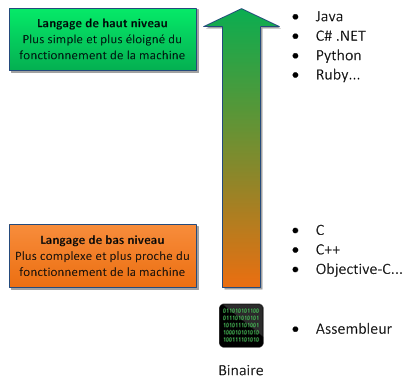
\includegraphics[scale=0.9]{Images/CPP}
\caption{Différents niveaux de langage informatique}
\label{fig:CPP}
\end{figure}

\section{Utilisation pratique}

% Processus de MASS
Nous venons de voir que quelque soit la co-simulation réalisée suivant le standard FMI, il est nécessaire d'importer un (ou plusieurs) FMU(s) sur le logiciel maître. La Figure \ref{fig:MASSProcessus} représente le processus d'échange et les fichiers nécessaires à la co-simulation entre EnergyPlus et le FMU MASS.

% Description des fichiers EnergyPlus
Pour faire une simulation sous EnergyPlus sans MASS, seulement deux fichiers d'entrée sont nécessaires. Le fichier *.idf, le fichier principal de la simulation qui contient les informations relatives aux bâtiments, aux systèmes et aux scénarios d'usages. Et le fichier *.epw, le fichier météo qui contient les données météorologiques heures par heures (la construction de ce type de fichier est présentée en section \ref{Météo}).

% Description des fichiers de MASS
Ces fichiers sont également nécessaires pour réaliser une co-simulation avec un FMU tel que MASS. En addition des deux fichiers EnergyPlus, deux fichiers sont obligatoires, le fichier de description des modèles et la bibliothèque de lien dynamique (DLL), ainsi qu'un ou plusieurs fichiers optionnels de configuration. Le fichier de description des modèles, appelé ModelDescription.xml dans MASS, contient les informations permettant de faire l'interface entre les données d'entrée et de sortie du logiciel maître EnergyPlus. Les données d'entrée de l'outil esclave étant les données de sortie du logiciel maître et les données de sortie de l'outil esclave étant les données de d'entrée du logiciel maître. La DLL contient le coeur de l'algorithme de la plateforme multi-agents MASS dans un format compatible avec EnergyPlus. Il est intéressant de noter que l'utilisation d'une bibliothèque dynamique est un excellent moyen pour réutiliser le code, économiser de l'espace dans les applications et mettre à jour la DLL sans recompiler toutes les applications. Enfin les fichiers de configuration permettent de configurer les informations relatives au FMU dans un fichier *.xml externe à EnergyPlus. Dans le cadre de MASS un seul et unique fichier de configuration, SimulationConfig.xml, est utilisé et comporte des informations sur les bâtiments, comme l'association des zones à des activités, et sur les agents, comme leur age, type d'activité et autres variables qui influent leurs comportements. Finalement, une fois ces trois fichiers intégrés à l'environnement de simulation, le fichier principal d'EnergyPlus *.idf doit être adapté à la co-simulation. Pour cela, le simulateur doit activer l'interface externe, définir le FMU lié à EnergyPlus, indiquer les variables d'entrée et de sortie (Pour plus de détails le lecteur peut se référer au guide d'application pour les interfaces externes d'EnergyPlus \cite{EP-ExternalInterface-16}).

\begin{figure}
\centering
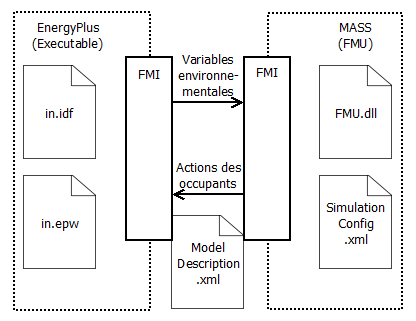
\includegraphics[scale=0.8]{Images/MASSProcessus}
\caption{Fichiers mis en jeu pour réaliser une co-simulation sous MASS et principe d'échange du FMI}
\label{fig:MASSProcessus}
\end{figure}

% Fonctions du FMI
D'un point de vu plus technique la Figure \ref{fig:diagramOfTheCo-Simulation}, reprise de Hong et al. \cite{Hong-16}, permet de présenter le processus et le fonctionnement interne du standard FMI. Lorsqu'EnergyPlus commence, il lit le fichier principal et détermine s'il est lié à un FMU. Si c'est le cas le maître EnergyPlus initialise le FMU grâce aux fonctions \textit{fmiInstantiateSlave} et \textit{fmiInitializeSlave}. Une fois ce pre-processus réalisé la co-simulation peut débuter et comporte trois phases. Premièrement, le FMU récupère les variables environnementales d'EnergyPlus sous la forme d'un tableau de valeurs, ensuite l'algorithme du FMU est parcouru grâce à la fonction \textit{fmiDoStep} (le processus interne de MASS est présenté en section \ref{FlowchartInternMASS}), puis dernièrement les résultats du pas de temps sont renvoyés au logiciel maître EnergyPlus avec la fonction \textit{fmiGetReal}. Une fois la fin de la simulation, la fonction \textit{fmiFreeSlaveInstance} est appelée pour libérer la mémoire occupée par le FMU MASS.

\begin{figure}
\centering
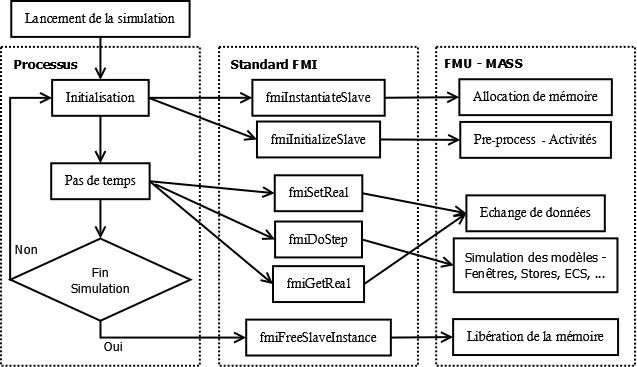
\includegraphics[scale=0.48]{Images/diagramOfTheCo-Simulation}
\caption{Diagramme de principe du fonctionnement interne du Standrd FMI en co-simulation}
\label{fig:diagramOfTheCo-Simulation}
\end{figure}

% Praticité d'utilisation
D'un point de vu pratique la génération des fichiers ModelDescription.xml et de la partie dédiée au FMU dans le fichier principal *.idf est optimisée par l'utilisation de scripts Python. Les modèles utilisés pour représenter le comportement des occupants étant stochastiques demandent d'être simulés plusieurs fois afin d'obtenir une répartition des résultats. Ces multi-simulations sont également lancées à l'aide d'un script Python, facilitant le travail du simulateur. Le traitement de l'ensemble des résultats issus des simulations est quant à lui traité grâce au langage R. Le point fort de R par rapport à un logiciel à menus déroulants réside dans la possibilité de programmer une suite d'analyses successive.

\section{Synthèse}

Suite aux choix réalisés et présentés dans les chapitres précédents sur l'utilisation de co-simulations d'un système multi-agents à un outils de STD, nous avons détaillé dans ce chapitre comment l'outil MASS développé initialement par l'Université de Nottingham fonctionne. Le choix de l'utilisation de \textit{Functional Mockup Interface} (FMI) plutôt que de \textit{Buildings Controls Virtual Test Bed} (BCVTB) est justifié par sa rapidité d'exécution. Le processus de fonctionnement du standard FMI est par la suite présenté en détail, avec notamment une description détaillée des fichiers relatifs aux FMUs.

Après avoir présenté dans cette section l'environnement de co-simulation, nous proposons dans le chapitre \ref{Modélisation du comportement des occupants}, d'exposer notre contribution à la plateforme SMA à agents réactifs tropiques MASS.

---- Il faut peut-être rajouter des Annexes pour présenter plus en détails les fichiers de MASS??? ---